%
% File: chap01.tex
% Author: Antigoni Kourou
% Description: Introduction chapter where the biology goes.
%
\let\textcircled=\pgftextcircled
\chapter{Introduction}
\label{chap:intro}
%
% General description of ICTs growth, etourism term and feedback systems
%

\initial{T}he exponential growth of Information and Communication Technologies (ICTs) has played a great role in the development of tourism industry. Electronic tourism (e-tourism) is the application of ICTs for tourism purposes, including the digitalization of all its processes and value chains \cite{buhalis2003etourism}. Increasingly, ICTs provide users with access to many sources of information and has eventually affected the consumer behavior in tourism industry \cite{mills2004handbook}. In order to remain a strong competitor, service providers have to keep their customers happy. Nowadays there is a huge variety of web services which provide a great complexity and diversity of recommended offers for meeting the demands of travelers. However, the personalized consumption patterns and individualistic lifestyles make it difficult for the service providers to anticipate tourists' behavior \cite{niemann2008enhancing}. For decision makers to successfully understand the requirements, needs, desires and preferences of the customer, detailed information has to be obtained. Travelers, making use of the ICT tools that facilitate the information retrieval and decision making processes, have now direct access to all types of information provided by tourism agencies, companies, marketers, enterprises or other users. Furthermore, ICTs and Internet have transformed e-tourism markets from customer-centric to customer-driven \cite{buhalis2011tourism}, meaning that users play a major role in creating and sharing traveling information through blogs and review websites. Online feedback mechanisms, also known as reputation systems, \textit{have emerged as a viable mechanism for fostering cooperation among strangers in such settings} \cite{dellarocas2003digitization}. Examples of these systems, for instance TripAdvisor, Booking.com or AirBnb, after each trade encourage both parties to give feedback about their trading partner based on their own experience. 
Customer feedback is an essential component in every modern business' tool kit. A big number customer feedback software tools exists for helping service providers to measure and improve customer satisfaction, identify unhappy customers, reduce churn and get valuable insight from customers. However, most of these tools are very expensive, considering that most of service providers can make use of their own feedback mechanisms.
%
\section{Problem statement}
% How feedback is collected and analyzed 
%
The most common types of consumer generated feedback are ratings from 1-5 stars and general text comments. An important separation exists between the distinct role of text comments as tacit knowledge and ratings as explicit knowledge and the ways they are analyzed. For online marketplaces to succeed, their feedback technologies must be able to not only collect users feedback, but to properly analyze it and utilize for decision making purposes \cite{pavlou2006nature}. However, current online travel systems, aiming to assist the consumer in finding suitable offers, filter the information based on location-price factor and on the overall ratings accumulated from the feedback system, meaning that text reviews are revealed for the public to read but they do not directly affect the overall analysis. Focusing on solely numerical ratings and ignoring the importance of text feedback leads to two major issues for feedback systems. 
%
% The issues with current analysis
% ---- BIAS -----
%

First, many academic papers on online reputation systems and building trust in the online marketplace report the existence of bias in online reviews \cite{bolton2013engineering,dellarocas2008sound,dini2009buying,fradkin2016bias,ghose2011estimating,resnick2006value}. {\color {red}{This bias is seen as a tendency of reviewers to systematically highly rate their experiences, thus reducing the difference between the ratings in the system and the true values is an important issue towards a more efficient online feedback system. These over-estimated high ratings create to the customers the idea of "perfection" in all directions, which doesn't leave room for discovering their possible negative features. Thus, utilizing only biased ratings produces many results that falsly clasify the listings as extremly good.}} On the other hand, the analysis of ratings does not indicate much information for the service providers, who aim to acquire knowledge on how to improve their services. In order to gain detailed insights from the feedback system, some service providers including Airbnb, ask its users to rate not only the overall quality of the listing, but also six accommodation features. However, since the overall ratings are biased \cite{fradkin2016bias}, how do we make sure that the ratings for specific features are objective? From this point of view, the bias on quantitative data of the system raises the issue of reliability on the system itself.

%
% ---- HIDDEN FEATURES -----
%

Second, the incompleteness of the analysis based solely in quantitative data leads to the need for complementary analysis. Customers' needs are considered multi-dimensional and difficult to measure on discrete scales such as ratings \cite{luo2005information}, therefore a customer has to extract the needed information from different sources and types of information provided by agencies, companies or other users. According to \cite{pavlou2006nature}, text comments are particularly interesting for the audience as a new trust-building means in online marketplaces by revealing hidden knowledge, which is often underestimated from their owners and cannot be described by negative/positive ratings. Furthermore, \cite{fradkin2016bias} suggests that text opinions influence the decision making process even when the ratings are high. In the Airbnb feedback system a negative rating is followed by a text in 45\% of the cases, which implies the great power of text analysis for discovering deeper insights for the listing \cite{fradkin2016bias}. Acknowledging the importance of text comments, some feedback systems often offer summaries to all text comments, which mostly consist on a bunch of most used words. However, this bag of words does not necessarily cover the features that a certain user is interested in, neither the features that need to be improved. The users or service providers still have to read all the text comments related to the feature, meaning that it still does not reduce much of the  work. A survey by \cite{pavlou2006institutional} asked the respondents to indicate how many feedback comments they examined before each online transaction. The result showed that 81\% reported examining 25 comments (one webpage), 5\% viewed 50 comments, 11\% more than 50 ones, and only 3\% did not examine any text comments. These findings reveal that despite the importance of text feedback to the users, it is difficult for them to access the meaning of numerous text comments \cite{pavlou2006institutional}. Given this situation, the average human reader will have difficulties on identifying and extracting the relevant information from the opinions in them. Automated analysis systems are thus needed \cite{liu2012sentiment}.
\section{Research question}
Natural language processing (NLP) enable computers to derive meaning from any human written input, including their opinions. The NLP methods for doing so fall into the category of sentiment mining methods, known also as \textit{opinion mining}. Examples of their application include mainly the movie rating systems (Netflix, IMDb) and the product rating systems (eBay). However, the importance of extracting sentiment of features from online reviews, besides their overall positive/negative sentiment is often ignored in the literature. This research proposes the implementation of feature-based opinion mining methods from complementing the analysis of customer feedback in e-tourism and accommodation market. The proposed approach uses an ontology based approach combined with sentiment mining techniques for generating opinion scores for each accommodation feature mentioned in the reviews of a feedback system. This solution deals with the two issues mentioned above, bias of ratings and the need for complementary text analysis for feature extraction. From its point of view, both issues can be brought together as one, since text analysis is believed to contribute to a better rating systems by reducing its bias \cite{fradkin2016bias}. By estimating sentiment scores for the text reviews, the pipeline transforms the text data into discrete quantitative form, which can easily be analyzed for different purposes. Thus, this paper focuses on two main questions:
\begin{quote} \textit{First, how can opinion mining methods be aligned with the quantitative data analysis in order to enhance focus on customer feedback and produce detailed analysis results?}

 \textit{And secondly, how good can feature-based opinion mining estimate the quality of accommodation features in e-tourism feedback systems?}
\end{quote}
By answering these two questions, the purpose of the paper is to offer to service providers a new reliable approach on enhancing focus on customers, based on users' generated content.

\section{Research rationale and structure}
Customer Focus Theory is one of the essential parts of Information Studies (IS) and it serves as a guidance for business on how to put focus on their customers, as their most valuable asset. From Figure \ref{fig:cusfoc} can be clearly seen that Customer Requirement, Information, Feedback and Relationships are the four key factors of a good focus on customer \cite{lohan2011examining}. In alignment with this guidance, businesses try their best on gathering customers information and feedback in several ways starting online forms, surveys and interviews to social media, forums and blogs. However, the most important part of work comes exactly after having the feedback, explicitly on how it is analyzed, interpreted and utilized. Most of business pay huge amount of money on outsourcing the feedback analysis, human resources (like the Amazon Mechanical Turk) and expensive software. From this point of view, the proposed approach is an added value for both service providers and their customer for several reasons. First, an analytic tool taking care of text feedback and bringing it into the traditional quantitative type of data, saves both a lot of time and money. Second, the insights and analysis are personalized to the business purposes, meaning that the winner is the one who gets the requirements properly. Thirdly, transforming text feedback into quantitative data serves as a measurable data-drive target over time, where businesses can check the quality directions of their services.
\begin{figure}[h!]
	\centering
	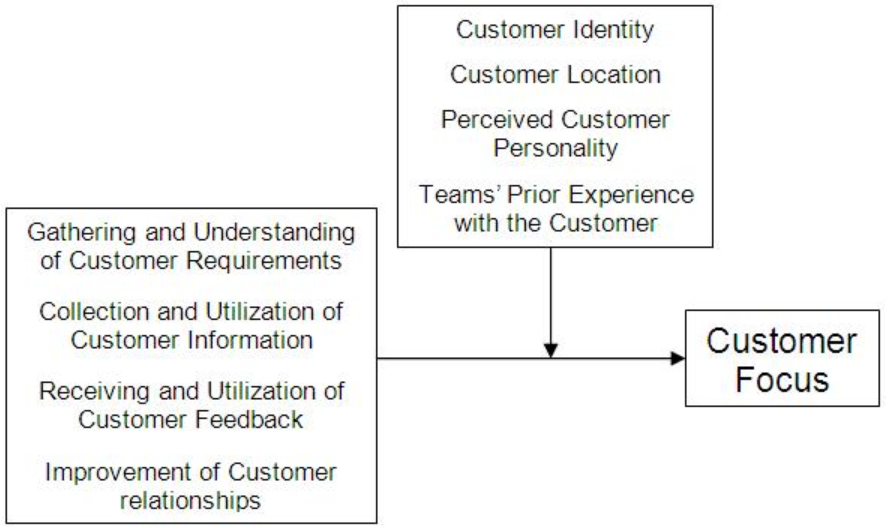
\includegraphics[height=0.25\textheight]{fig01/CustomerFocus}
	\caption{Customer Focus Theory. Source: \cite{lohan2011examining}}
	\label{fig:cusfoc}
\end{figure}

From the literature point of view, it is noticed a gap in the alignment between text analysis with the analysis from quantitative data. This paper adds value firstly to the Customer Focus Theory and secondly to the use of feature-based opinion mining for analysis purposes. The existing systems and methods of feature-based opinion are examined and presented in the following chapter. Shortly, we can conclude that the literature lacks a system where all the features belonging to a certain domain are analyzed and scored discretely based on text feedback. Furthermore, many reviewed papers\cite{fradkin2016bias,liu2012sentiment,pavlou2006nature,yaakub2012integration,zhang2012weakness,dellarocas2008sound}  suggest the use of sentiment analysis for complementing the data analysis in feedback systems as an area in need for further research.

To provide an answer to the research questions, this paper is organized in seven chapters. The importance of gathering and analyzing customer feedback is introduced by the first part of the paper and it is followed, in the second chapter, by the current state-of-the-art of feature-based opinion mining used for analyzing customer feedback. The proposed approach is discussed in the third chapter by explaining each step of the pipeline developed for this research. The fourth chapter covers the methodology used in the research, from collecting the data to the analysis of the output. In chapter five, the whole proposed approach is evaluated in comparison to ratings given by humans. Afterwards the results are presented and visualized, which leads the discussion to the limitations of this work, its implications and further work to be done. Finally the paper concludes with a recap of the main findings. 